\documentclass[11pt, a4paper]{MATH2023}
\usepackage{fancyhdr}
\usepackage{setspace}
\usepackage{amsmath,mathrsfs}
\usepackage{multicol}
\usepackage{amssymb}
\usepackage{graphicx}
\usepackage{caption}
\usepackage{subcaption}
\usepackage{xcolor}
\usepackage{enumitem}
\usepackage{tikz}
\usepackage{mathtools}
\usetikzlibrary{matrix}
\usepackage[normalem]{ulem}
\usepackage{multirow}
\usepackage[linesnumbered, ruled, boxed]{algorithm2e}
\SetKwRepeat{Do}{do}{while}
\newcommand{\eg}{\textbf{[Example.] }}
\newcommand{\sol}{\textbf{[Solution.] }}
\newcommand{\vct}{\underline}
\newcommand{\vv}{\underline{v}}
\newcommand{\uu}{\underline{u}}
\newcommand{\ww}{\underline{w}}
\newcommand{\rr}{\underline{r}}
\newcommand{\ii}{\underline{i}}
\newcommand{\kk}{\underline{k}}
\newcommand{\jj}{\underline{j}}
\newcommand{\va}{\underline{a}}
\newcommand{\bb}{\underline{b}}
\newcommand{\cc}{\underline{c}}
\newcommand{\dd}{\underline{d}}

\title{Chapter 14}
\subtitle{Multiple Integrations}

\begin{document}
\begin{spacing}{1.3}

    \section{Double Integrals Over Rectangles}

    Recall that in single variable calculus, we divided a region into 
    thin rectangles and use the {\bf Riemann Sum} as integral.
    \begin{center}
        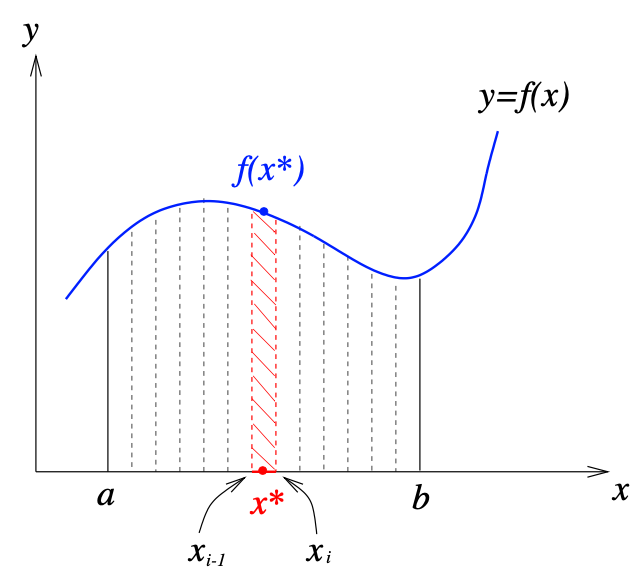
\includegraphics[scale=0.35]{images/Ch14-intro.png}
    \end{center}
    $$\int_a^b f(x)dx=\lim_{n\rightarrow \infty}\sum_{i=1}^n f(x_i^\star)\delta x_i$$
    
    Actually, instead of thin rectangles, we can use {\it small rectangles} to cover the area.

    \eg Find the area bounded by $y=x$, $x=1$ and $y=0$.

    \sol (1) View the area as bounded by {\it upper curve} and {\it lower curve}.
    

    \tikzset{every picture/.style={line width=0.75pt}} %set default line width to 0.75pt        
    \begin{center}
        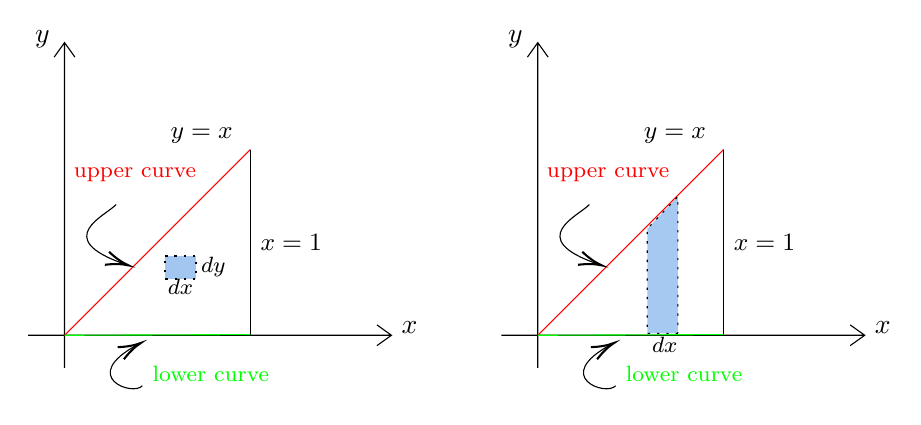
\begin{tikzpicture}[x=0.75pt,y=0.75pt,yscale=-1,xscale=1]
            %uncomment if require: \path (0,300); %set diagram left start at 0, and has height of 300
        
            %Shape: Axis 2D [id:dp3896868200656678] 
            \draw  (68,207) -- (243,207)(85.5,66) -- (85.5,222.67) (236,202) -- (243,207) -- (236,212) (80.5,73) -- (85.5,66) -- (90.5,73)  ;
            %Straight Lines [id:da8649162174794645] 
            \draw [color={rgb, 255:red, 255; green, 0; blue, 0 }  ,draw opacity=1 ]   (85.5,207) -- (175,117.5) ;
            %Straight Lines [id:da8918167425471388] 
            \draw    (175,117.5) -- (175,206.67) ;
            %Straight Lines [id:da20672609799626906] 
            \draw [color={rgb, 255:red, 0; green, 255; blue, 0 }  ,draw opacity=1 ]   (85.5,207) -- (175,206.67) ;
            %Curve Lines [id:da7341114132390345] 
            \draw    (110.33,144) .. controls (105.74,149.25) and (78.5,160.33) .. (114.64,172.76) ;
            \draw [shift={(116.33,173.33)}, rotate = 198.14] [color={rgb, 255:red, 0; green, 0; blue, 0 }  ][line width=0.75]    (10.93,-3.29) .. controls (6.95,-1.4) and (3.31,-0.3) .. (0,0) .. controls (3.31,0.3) and (6.95,1.4) .. (10.93,3.29)   ;
            %Curve Lines [id:da6058369715667598] 
            \draw    (123,231.33) .. controls (118.4,236.59) and (91.81,226.96) .. (120.96,211.38) ;
            \draw [shift={(122.33,210.67)}, rotate = 512.95] [color={rgb, 255:red, 0; green, 0; blue, 0 }  ][line width=0.75]    (10.93,-3.29) .. controls (6.95,-1.4) and (3.31,-0.3) .. (0,0) .. controls (3.31,0.3) and (6.95,1.4) .. (10.93,3.29)   ;
            %Shape: Rectangle [id:dp5051745743053773] 
            \draw  [color={rgb, 255:red, 0; green, 0; blue, 0 }  ,draw opacity=1 ][fill={rgb, 255:red, 74; green, 144; blue, 226 }  ,fill opacity=0.51 ][dash pattern={on 0.84pt off 2.51pt}][line width=0.75]  (134,168.67) -- (149,168.67) -- (149,180) -- (134,180) -- cycle ;
            %Shape: Axis 2D [id:dp8934264331658603] 
            \draw  (296,207) -- (471,207)(313.5,66) -- (313.5,222.67) (464,202) -- (471,207) -- (464,212) (308.5,73) -- (313.5,66) -- (318.5,73)  ;
            %Straight Lines [id:da7529215091369386] 
            \draw [color={rgb, 255:red, 255; green, 0; blue, 0 }  ,draw opacity=1 ]   (313.5,207) -- (403,117.5) ;
            %Straight Lines [id:da6761798304849251] 
            \draw    (403,117.5) -- (403,206.67) ;
            %Straight Lines [id:da16391256653051056] 
            \draw [color={rgb, 255:red, 0; green, 255; blue, 0 }  ,draw opacity=1 ]   (313.5,207) -- (403,206.67) ;
            %Curve Lines [id:da35417352536646507] 
            \draw    (338.33,144) .. controls (333.74,149.25) and (306.5,160.33) .. (342.64,172.76) ;
            \draw [shift={(344.33,173.33)}, rotate = 198.14] [color={rgb, 255:red, 0; green, 0; blue, 0 }  ][line width=0.75]    (10.93,-3.29) .. controls (6.95,-1.4) and (3.31,-0.3) .. (0,0) .. controls (3.31,0.3) and (6.95,1.4) .. (10.93,3.29)   ;
            %Curve Lines [id:da5929159990416739] 
            \draw    (351,231.33) .. controls (346.4,236.59) and (319.81,226.96) .. (348.96,211.38) ;
            \draw [shift={(350.33,210.67)}, rotate = 512.95] [color={rgb, 255:red, 0; green, 0; blue, 0 }  ][line width=0.75]    (10.93,-3.29) .. controls (6.95,-1.4) and (3.31,-0.3) .. (0,0) .. controls (3.31,0.3) and (6.95,1.4) .. (10.93,3.29)   ;
            %Shape: Trapezoid [id:dp507673701497652] 
            \draw  [fill={rgb, 255:red, 74; green, 144; blue, 226 }  ,fill opacity=0.49 ][dash pattern={on 0.84pt off 2.51pt}] (381,206.11) -- (366.25,206.11) -- (366.25,155.72) -- (381,140.15) -- cycle ;
        
            % Text Node
            \draw (70,59.07) node [anchor=north west][inner sep=0.75pt]    {$y$};
            % Text Node
            \draw (246.67,199.07) node [anchor=north west][inner sep=0.75pt]    {$x$};
            % Text Node
            \draw (135.33,105.73) node [anchor=north west][inner sep=0.75pt]  [font=\small]  {$y=x$};
            % Text Node
            \draw (178.67,157.4) node [anchor=north west][inner sep=0.75pt]  [font=\small]  {$x=1$};
            % Text Node
            \draw (88.67,125.33) node [anchor=north west][inner sep=0.75pt]  [color={rgb, 255:red, 255; green, 0; blue, 0 }  ,opacity=1 ] [align=left] {{\footnotesize upper curve}};
            % Text Node
            \draw (126.67,220.67) node [anchor=north west][inner sep=0.75pt]  [color={rgb, 255:red, 0; green, 255; blue, 0 }  ,opacity=1 ] [align=left] {{\footnotesize lower curve}};
            % Text Node
            \draw (134,178.73) node [anchor=north west][inner sep=0.75pt]  [font=\footnotesize]  {$dx$};
            % Text Node
            \draw (150,168.07) node [anchor=north west][inner sep=0.75pt]  [font=\footnotesize]  {$dy$};
            % Text Node
            \draw (298,59.07) node [anchor=north west][inner sep=0.75pt]    {$y$};
            % Text Node
            \draw (474.67,199.07) node [anchor=north west][inner sep=0.75pt]    {$x$};
            % Text Node
            \draw (363.33,105.73) node [anchor=north west][inner sep=0.75pt]  [font=\small]  {$y=x$};
            % Text Node
            \draw (406.67,157.4) node [anchor=north west][inner sep=0.75pt]  [font=\small]  {$x=1$};
            % Text Node
            \draw (316.67,125.33) node [anchor=north west][inner sep=0.75pt]  [color={rgb, 255:red, 255; green, 0; blue, 0 }  ,opacity=1 ] [align=left] {{\footnotesize upper curve}};
            % Text Node
            \draw (354.67,220.67) node [anchor=north west][inner sep=0.75pt]  [color={rgb, 255:red, 0; green, 255; blue, 0 }  ,opacity=1 ] [align=left] {{\footnotesize lower curve}};
            % Text Node
            \draw (367.33,206.73) node [anchor=north west][inner sep=0.75pt]  [font=\footnotesize]  {$dx$};
        \end{tikzpicture}
    \end{center}
    

    For the {\it small rectangles} with $dA=dxdy=dydx$, we first move it vertically,
    the lower bound is $y=0$, and the upper bound is $y=x$, hence $\disp \int_0^x dy$
    is the shaded area in right image above.

    Then we move the shaded area horizontally, the left bound is point $x=0$, while 
    the right bound is point $x=1$, thus the total area is: 
    $$A=\int_0^1 \int_0^x dydx=\left. \int_0^1 y \right\vert_0^x dx=\int_0^1 xdx=\frac{1}{2}$$

    (2) Alternatively, we can first move the rectangle horizontally, hitting 
    {\it left curve} $x=y$ and {\it right curve} $x=1$, hence the shaded area is 
    $\disp \int_y^1 dx$. {\red note here we integral $dx$ first, so when hitting 
    the boundaries, we need to check $x$ equals to what, i.e. $x=f(y)$.}
    For example, here the two bounds are $x=y$ and $x=1$.
    \begin{center}
        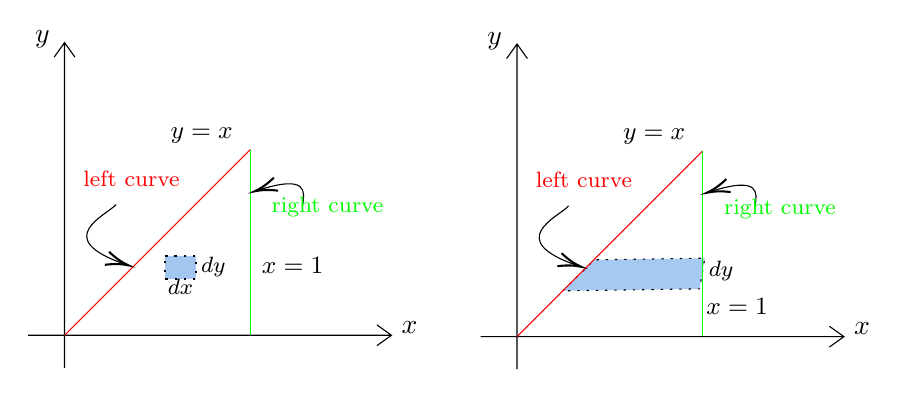
\begin{tikzpicture}[x=0.75pt,y=0.75pt,yscale=-1,xscale=1]
        %uncomment if require: \path (0,300); %set diagram left start at 0, and has height of 300

        %Shape: Axis 2D [id:dp7553906893045521] 
        \draw  (88,227) -- (263,227)(105.5,86) -- (105.5,242.67) (256,222) -- (263,227) -- (256,232) (100.5,93) -- (105.5,86) -- (110.5,93)  ;
        %Straight Lines [id:da35403404535445815] 
        \draw [color={rgb, 255:red, 255; green, 0; blue, 0 }  ,draw opacity=1 ]   (105.5,227) -- (195,137.5) ;
        %Straight Lines [id:da01645345984200941] 
        \draw [color={rgb, 255:red, 0; green, 255; blue, 0 }  ,draw opacity=1 ][fill={rgb, 255:red, 0; green, 255; blue, 0 }  ,fill opacity=1 ]   (195,137.5) -- (195,226.67) ;
        %Curve Lines [id:da1854977378917313] 
        \draw    (130.33,164) .. controls (125.74,169.25) and (98.5,180.33) .. (134.64,192.76) ;
        \draw [shift={(136.33,193.33)}, rotate = 198.14] [color={rgb, 255:red, 0; green, 0; blue, 0 }  ][line width=0.75]    (10.93,-3.29) .. controls (6.95,-1.4) and (3.31,-0.3) .. (0,0) .. controls (3.31,0.3) and (6.95,1.4) .. (10.93,3.29)   ;
        %Curve Lines [id:da04722306457844705] 
        \draw    (220.33,163.67) .. controls (220.98,157.82) and (222.9,149.43) .. (198.9,157.05) ;
        \draw [shift={(197,157.67)}, rotate = 341.57] [color={rgb, 255:red, 0; green, 0; blue, 0 }  ][line width=0.75]    (10.93,-3.29) .. controls (6.95,-1.4) and (3.31,-0.3) .. (0,0) .. controls (3.31,0.3) and (6.95,1.4) .. (10.93,3.29)   ;
        %Shape: Rectangle [id:dp32583575696458844] 
        \draw  [color={rgb, 255:red, 0; green, 0; blue, 0 }  ,draw opacity=1 ][fill={rgb, 255:red, 74; green, 144; blue, 226 }  ,fill opacity=0.51 ][dash pattern={on 0.84pt off 2.51pt}][line width=0.75]  (154,188.67) -- (169,188.67) -- (169,200) -- (154,200) -- cycle ;
        %Shape: Trapezoid [id:dp3210513944610718] 
        \draw  [fill={rgb, 255:red, 74; green, 144; blue, 226 }  ,fill opacity=0.49 ][dash pattern={on 0.84pt off 2.51pt}] (345.54,205.61) -- (360.82,190.64) -- (413.98,189.86) -- (411.49,204.65) -- cycle ;
        %Shape: Axis 2D [id:dp46120188682750873] 
        \draw  (306,227.67) -- (481,227.67)(323.5,86.67) -- (323.5,243.33) (474,222.67) -- (481,227.67) -- (474,232.67) (318.5,93.67) -- (323.5,86.67) -- (328.5,93.67)  ;
        %Straight Lines [id:da22273680492149706] 
        \draw [color={rgb, 255:red, 255; green, 0; blue, 0 }  ,draw opacity=1 ]   (323.5,227.67) -- (413,138.17) ;
        %Straight Lines [id:da8910127482619856] 
        \draw [color={rgb, 255:red, 0; green, 255; blue, 0 }  ,draw opacity=1 ][fill={rgb, 255:red, 0; green, 255; blue, 0 }  ,fill opacity=1 ]   (413,138.17) -- (413,227.33) ;
        %Curve Lines [id:da6790580082651905] 
        \draw    (348.33,164.67) .. controls (343.74,169.92) and (316.5,180.99) .. (352.64,193.43) ;
        \draw [shift={(354.33,194)}, rotate = 198.14] [color={rgb, 255:red, 0; green, 0; blue, 0 }  ][line width=0.75]    (10.93,-3.29) .. controls (6.95,-1.4) and (3.31,-0.3) .. (0,0) .. controls (3.31,0.3) and (6.95,1.4) .. (10.93,3.29)   ;
        %Curve Lines [id:da2701777279829498] 
        \draw    (438.33,164.33) .. controls (438.98,158.48) and (440.9,150.1) .. (416.9,157.72) ;
        \draw [shift={(415,158.33)}, rotate = 341.57] [color={rgb, 255:red, 0; green, 0; blue, 0 }  ][line width=0.75]    (10.93,-3.29) .. controls (6.95,-1.4) and (3.31,-0.3) .. (0,0) .. controls (3.31,0.3) and (6.95,1.4) .. (10.93,3.29)   ;

        % Text Node
        \draw (90,79.07) node [anchor=north west][inner sep=0.75pt]    {$y$};
        % Text Node
        \draw (266.67,219.07) node [anchor=north west][inner sep=0.75pt]    {$x$};
        % Text Node
        \draw (155.33,125.73) node [anchor=north west][inner sep=0.75pt]  [font=\small]  {$y=x$};
        % Text Node
        \draw (199.33,188.07) node [anchor=north west][inner sep=0.75pt]  [font=\small]  {$x=1$};
        % Text Node
        \draw (113.33,146.67) node [anchor=north west][inner sep=0.75pt]  [color={rgb, 255:red, 255; green, 0; blue, 0 }  ,opacity=1 ] [align=left] {{\footnotesize left curve}};
        % Text Node
        \draw (204,159.33) node [anchor=north west][inner sep=0.75pt]  [color={rgb, 255:red, 0; green, 255; blue, 0 }  ,opacity=1 ] [align=left] {{\footnotesize right curve}};
        % Text Node
        \draw (154,198.73) node [anchor=north west][inner sep=0.75pt]  [font=\footnotesize]  {$dx$};
        % Text Node
        \draw (170,188.07) node [anchor=north west][inner sep=0.75pt]  [font=\footnotesize]  {$dy$};
        % Text Node
        \draw (414.65,189.92) node [anchor=north west][inner sep=0.75pt]  [font=\footnotesize]  {$dy$};
        % Text Node
        \draw (308,79.73) node [anchor=north west][inner sep=0.75pt]    {$y$};
        % Text Node
        \draw (484.67,219.73) node [anchor=north west][inner sep=0.75pt]    {$x$};
        % Text Node
        \draw (373.33,126.4) node [anchor=north west][inner sep=0.75pt]  [font=\small]  {$y=x$};
        % Text Node
        \draw (413.49,208.05) node [anchor=north west][inner sep=0.75pt]  [font=\small]  {$x=1$};
        % Text Node
        \draw (331.33,147.33) node [anchor=north west][inner sep=0.75pt]  [color={rgb, 255:red, 255; green, 0; blue, 0 }  ,opacity=1 ] [align=left] {{\footnotesize left curve}};
        % Text Node
        \draw (422,160) node [anchor=north west][inner sep=0.75pt]  [color={rgb, 255:red, 0; green, 255; blue, 0 }  ,opacity=1 ] [align=left] {{\footnotesize right curve}};
        \end{tikzpicture}
    \end{center}

    Then we move the shaded area vertically, hitting lower bound $y=0$(a point) and upper bound $y=1$(a point),
    hence the total area is: 
    $$A=\int_0^1 \int_y^1 dxdy=\left.\int_0^1  x \right\vert_y^1 dy=\int_0^1(1-y)dy=\frac{1}{2}$$

    \section{Double Integrals Over General Regions}

    \section{Double Integrals in Polar Coordinates}


    \newpage
    \section{Change of Variables in Integrals}

    Recall that in single variable calculus, we often use a {\it substitution} to simplify an integral.
    $$\int_a^b f(x)dx=\int_c^df(g(u))\cdot g'(u)\ du$$
    where $a=g(c)$ and $b=g(d)$. Notice that we can {\it view substitution as a kind of mapping}, and 
    the change-of-variable process introduces {\it an additional factor} $g'(u)$ into the integrand.

    This method can also be useful in multiple integrals. We have already seen one example: integration 
    in {\it polar coordinate}.
    $$\iint_{R} f(x, y) d A_{x y}=\iint_{S} f(r \cos \theta, r \sin \theta) r d r d \theta=\iint_{S} f(r \cos \theta, r \sin \theta) r d A_{r \theta}$$
    In this example, {\it the additional factor} is $r$.

    The {\it mapping} $T$ is shown as below: we transform the region $R$ into $S$, where $S$ is an rectangle in 
    $\theta r$-plane, which is easy to integrate.
    \begin{center}
        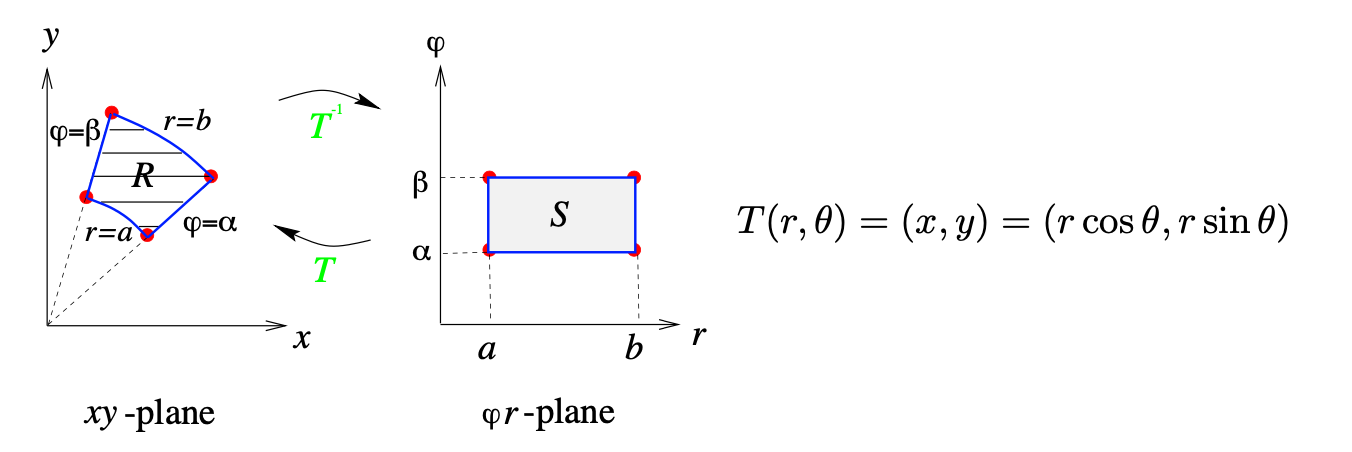
\includegraphics[scale=0.55]{images/Ch14-jacobians-polar-mapping.png}
    \end{center}

    \newpage
    \eg Find a change of variable.

    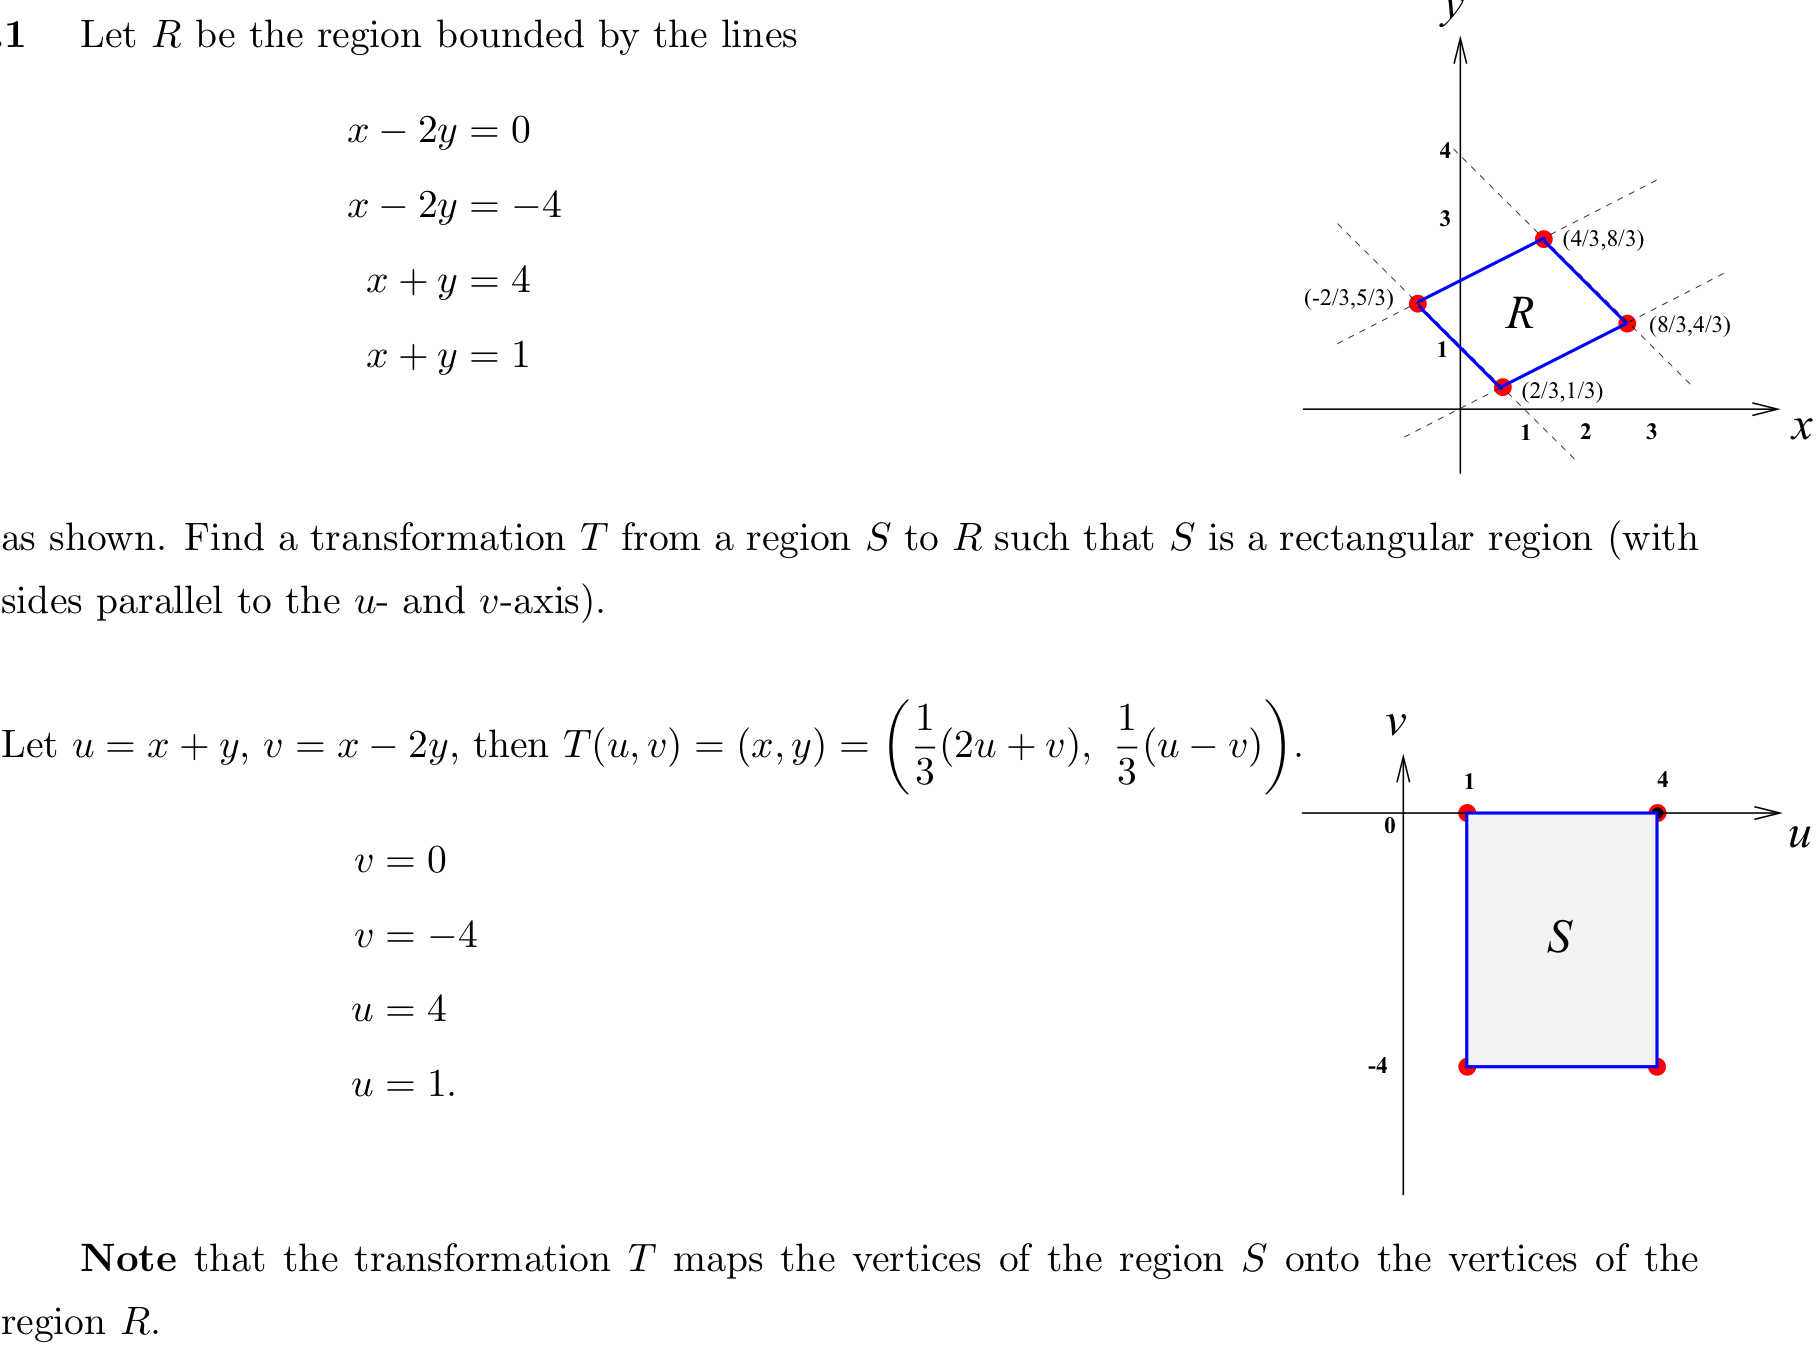
\includegraphics[scale=0.25]{images/Ch14-change-var-eg.jpeg}

    Now, to find $\disp \iint_R f(x,y) dxdy$, if we make the change of variables $x=g(u,v), y=h(u,v)$,
    then {\it we are mapping things in uv-plane onto things in xy-plane}. For mapping function 
    $T(u,v)=(g(u,v), h(u,v))=(x,y)$, and assume the area $S$ in $uv$-plane corresponds 
    to region $R$ in $xy$-plane, as shown below.

    \begin{center}
        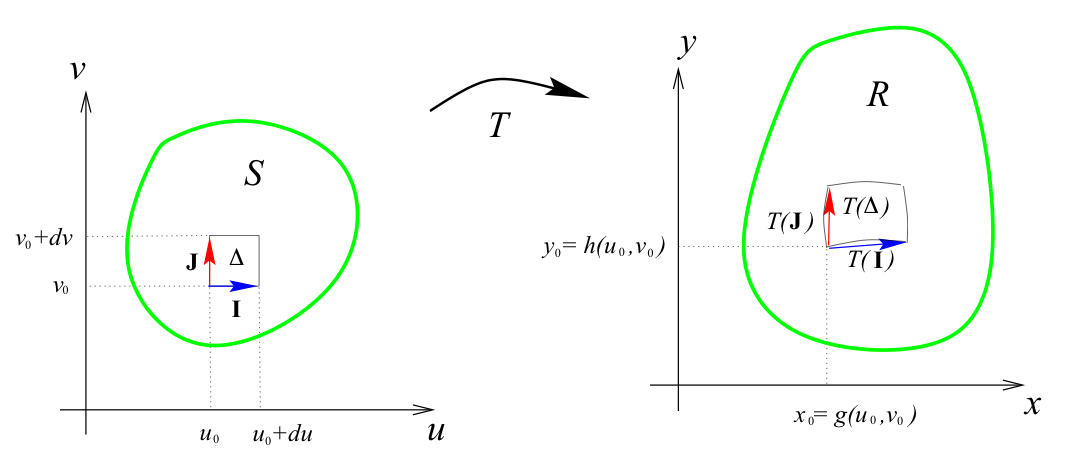
\includegraphics[scale=0.33]{images/Ch14-jacobian-mapping.jpeg}
    \end{center}

    We still use the method that integrate all ``small rectangles'', $\Delta$, as shown in $uv$-plane.
    Assume $\Delta$ locates at $(u_0,v_0)$ and has area $dA=dudv$. Let

    $\bf I$ be the vector from $\left(u_{0}, v_{0}\right)$ to $\left(u_{0}+d u, v_{0}\right)$ and\\
    $\mathbf{J}$ be the vector from $\left(u_{0}, v_{0}\right)$ to $\left(u_{0}, v_{0}+d v\right)$. 
    
    Then mapping $T$ ``takes'' $\bf I$ to the vector $T(\mathbf{I})$ from 
    $\left(g\left(u_{0}, v_{0}\right), h\left(u_{0}, v_{0}\right)\right)$ to 
    $\left(g\left(u_{0}+d u, v_{0}\right), h\left(u_{0}+d u, v_{0}\right)\right)$. 
    Notice the vector $T({\bf I})$ is {\it not necessary a straight vector}. Now
    $$
    \begin{aligned}
    T(\mathbf{I}) &=\left(g\left(u_{0}+d u, v_{0}\right)-g\left(u_{0}, v_{0}\right), h\left(u_{0}+d u, v_{0}\right)-h\left(u_{0}, v_{0}\right)\right) \\
    &=\left(\frac{g\left(u_{0}+d u, v_{0}\right)-g\left(u_{0}, v_{0}\right)}{d u}, \frac{h\left(u_{0}+d u, v_{0}\right)-h\left(u_{0}, v_{0}\right)}{d u}\right) d u \\
    &=\left(\frac{\partial g}{\partial u}, \frac{\partial h}{\partial u}\right) d u 
    \ \ {\rm \blue (for\ } {\blue  du\rightarrow 0)}
    \end{aligned}
    $$
    Similarly, $\disp T(\mathbf{J})=\left(\frac{\partial g}{\partial v}, \frac{\partial h}{\partial v}\right) dv$. 
    
    Then the area of $T(\Delta)$ is
    $$
    d x d y =\left\| T({\rm I})\cdot T({\rm J}) \right\|=\left| \left|\begin{array}{ll}
    \frac{\partial x}{\partial u} & \frac{\partial y}{\partial u} \\
    \frac{\partial x}{\partial v} & \frac{\partial y}{\partial v}
    \end{array}\right| d u d v\right|=\left| \frac{\partial x}{\partial u} \frac{\partial y}{\partial v}-\frac{\partial x}{\partial v} \frac{\partial y}{\partial u} \right| d u d v
    $$

    which means, $dA_{xy}=|J|\ dA_{uv}$, where $|J|$ is the ``additional factor'' caused by this substitution,
    and it is called the {\bf Jacobian} of mapping $T$, given by: 
    \begin{center}
        \boxed{$$\disp T=\frac{\partial(x, y)}{\partial(u, v)}
        =\frac{\partial x}{\partial u} \frac{\partial y}{\partial v}-\frac{\partial x}{\partial v} \frac{\partial y}{\partial u}
        =\left|\begin{array}{ll}\frac{\partial x}{\partial u} & \frac{\partial x}{\partial v} \\ \frac{\partial y}{\partial u} & \frac{\partial y}{\partial v}\end{array}\right|$$}
    \end{center}

    Therefore, the formula of {\it change of variable for two variables} is: 
    \begin{center}
        \boxed{
            $$\disp \iint_{R=T(S)} f(x, y) d x d y=\iint_{S} f(T(u, v))\left|\frac{\partial(x, y)}{\partial(u, v)}\right| d u d v$$
        }
    \end{center}
    

    while for {\it three variables}, 
    \begin{center}
        \boxed{
            $$\disp \iiint_{R=T(S)} f(x, y, z) d x d y d z=
            \iiint_{S} f(T(u, v, w))\left|\frac{\partial(x, y, z)}{\partial(u, v, w)}\right| d u d v d w$$
        }
    \end{center}

    \newpage
    \eg Find the area of $\disp \frac{x^2}{a^2}+\frac{y^2}{b^2}=1$.

    \sol {\bf Method 1:} directly integrate 
    \begin{align*}
        \frac{1}{4}A &= \int_{0}^{a} \int_{0}^{b\sqrt{1-\frac{x^2}{a^2}}}\ dydx\\
         &= \int_0^a b\sqrt{1-\frac{x^2}{a^2}}\ dx
    \end{align*}

    We are familiar with substitution in single variable integration, let $x=a\sin\theta$,
    when $x=0$, $\theta=0$, and when $x=a$, $\theta=\dfrac{\pi}{2}$. Then,
    \begin{align*}
        \frac{1}{4}A &= \int_0^{\frac{\pi}{2}} b(1-\sin^2\theta)^{\frac{1}{2}} a\cos\theta\ d\theta \\ 
        &= ab\int_0^{\frac{\pi}{2}} \cos^2\theta\ d\theta\\
        &= ab\int_0^{\frac{\pi}{2}} \frac{1}{2}(1-\cos2\theta)\ d\theta\\
        &= \frac{1}{4}ab\pi
    \end{align*}

    {\bf Method 2:} Mapping the ellipse to a disk.

    Let $x=au,\ y=bv$, then $\disp \frac{x^2}{a^2}+\frac{y^2}{b^2}=1$ becomes $u^2+v^2=1$.

    The Jacobian of this mapping 
    $$J=\left|\begin{array}{ll}\frac{\partial x}{\partial u} & \frac{\partial x}{\partial v} \\ \frac{\partial y}{\partial u} & \frac{\partial y}{\partial v}\end{array}\right|
    =\left| \begin{array}{cc}
        a & 0 \\ 0 & b
    \end{array} \right|=ab$$

    Therefore, the area of ellipse 
    $$\iint_R\ dA_{xy}=\iint_S\ J\cdot dA_{xy}=\iint_S\ ab\ dA_{uv}=ab\pi$$

    We observe that method 2 is much easier than method 1.

    \newpage
    \eg Find the area bounded by $\sqrt[4]{x}+\sqrt[4]{y}=1$ and the $x$ and $y$ axes.

    \sol

    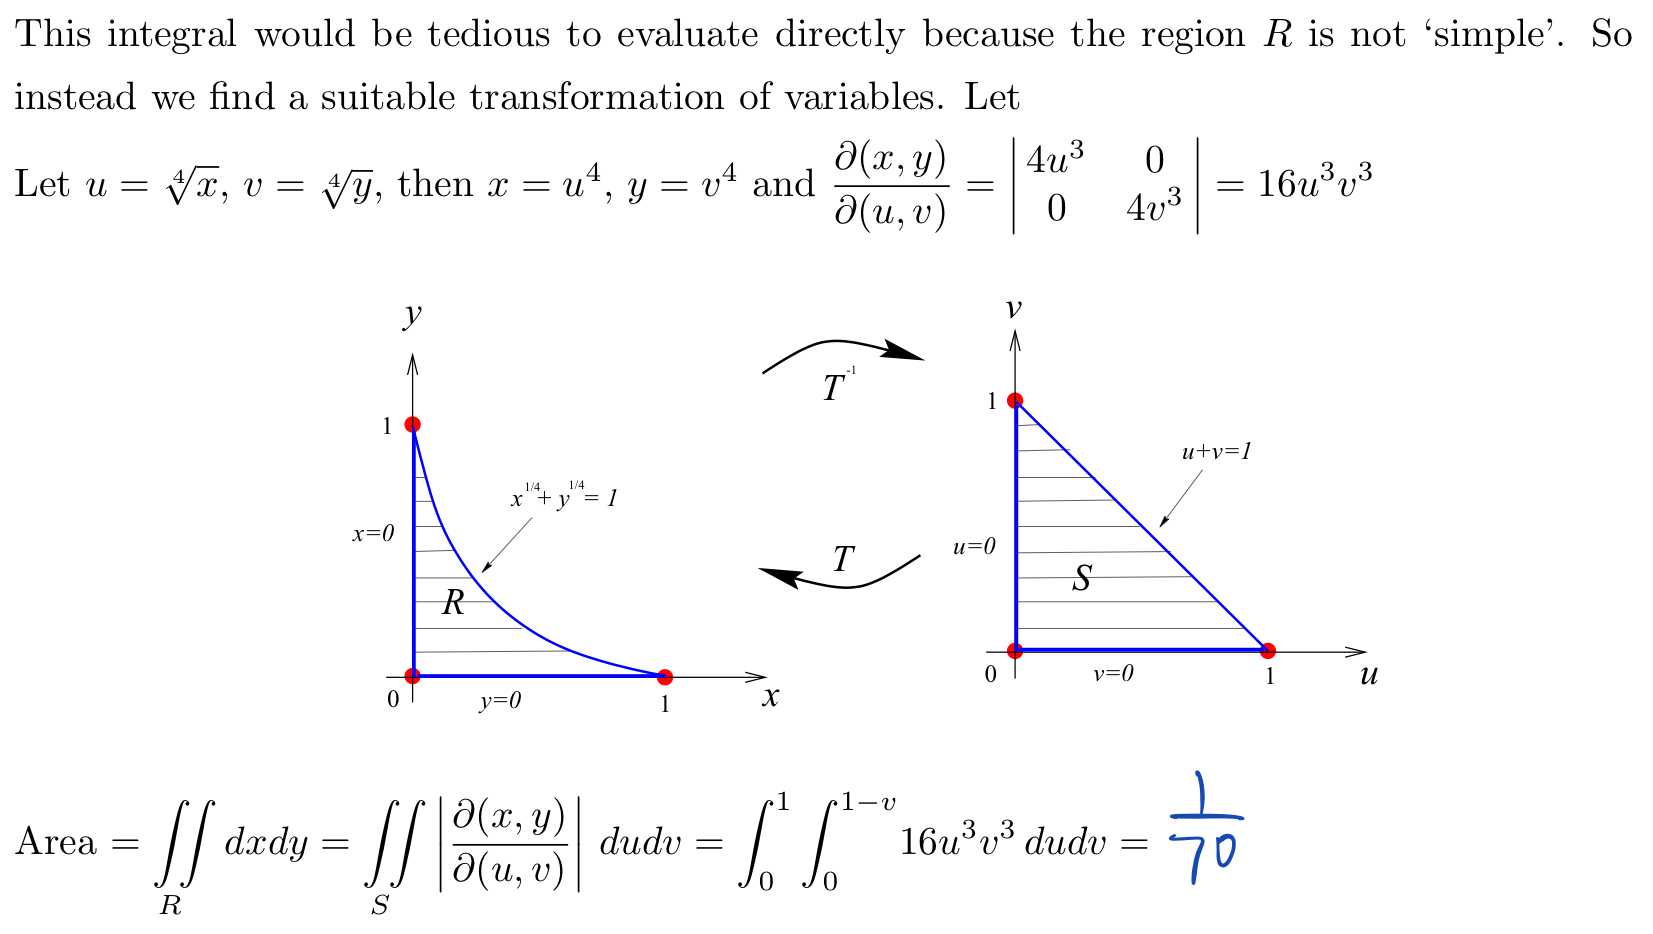
\includegraphics[scale=0.24]{images/Ch14-jacobian-eg2.jpeg}

    \vspace{0.2in}
    Sometimes, it's not easy to calculate $\dfrac{\partial(x, y)}{\partial(u, v)}$, 
    since usually we substitute $u$ and $v$ as functions of $x$ and $y$, so we always need to find the inverse 
    function in order to calculate $\dfrac{\partial(x, y)}{\partial(u, v)}$. So we consider the relationship 
    between  $\dfrac{\partial(x, y)}{\partial(u, v)}$ and $\dfrac{\partial(u, v)}{\partial(x, y)}$.

    Because of $\det A \det B=\det(AB)$, 
    \begin{align*}
        \frac{\partial(x, y)}{\partial(u, v)} \cdot \frac{\partial(u, v)}{\partial(x, y)} 
        &= \left|\begin{array}{ll}\frac{\partial x}{\partial u} & \frac{\partial x}{\partial v} \\ 
            \frac{\partial y}{\partial u} & \frac{\partial y}{\partial v}\end{array} \right| 
            \left|  \begin{array}{ll}\frac{\partial u}{\partial x} & \frac{\partial u}{\partial y} \\ 
                \frac{\partial v}{\partial x} & \frac{\partial v}{\partial y}\end{array}\right|\\
        &= \left|\begin{array}{ll}\frac{\partial x}{\partial u} \frac{\partial u}{\partial x}+\frac{\partial x}{\partial v} \frac{\partial v}{\partial x} & 
            \frac{\partial x}{\partial u} \frac{\partial u}{\partial y}+\frac{\partial x}{\partial v} \frac{\partial v}{\partial y} \\ 
            \frac{\partial y}{\partial u} \frac{\partial u}{\partial x}+\frac{\partial y}{\partial v} \frac{\partial v}{\partial x} & 
            \frac{\partial y}{\partial u} \frac{\partial u}{\partial y}+\frac{\partial y}{\partial v} \frac{\partial v}{\partial y}\end{array}\right| \\ 
        &=\left|\begin{array}{ll}\frac{\partial x}{\partial x} & \frac{\partial x}{\partial y} \\ 
                \frac{\partial y}{\partial x} & \frac{\partial y}{\partial y}\end{array}\right|
        =\left|\begin{array}{cc}1 & 0 \\ 0 & 1\end{array}\right|=1
    \end{align*}

    Therefore, if $x(u,v)$ and $y(u,v)$ have continuous first partial derivatives, and that 
    $$\frac{\partial(x, y)}{\partial(u, v)} \neq 0 \quad \text { at } \quad(u, v) \quad \text { (one-to-one map). }$$
    Then
    \begin{center}
        \boxed{$$\disp \frac{\partial(x, y)}{\partial(u, v)}=\frac{1}{\dfrac{\partial(u, v)}{\partial(x, y)}}$$}
    \end{center}

    \newpage
    \eg Find $\disp \iint_{A}\left(x^{2}+y^{2}\right) d x d y$, 
    where $A=\left[(x, y) \mid x, y>0, \quad 2 \leqslant x^{2}-y^{2} \leqslant 4, \quad \frac{1}{2} \leqslant x y \leqslant \frac{3}{2}\right]$

    \sol 
    
    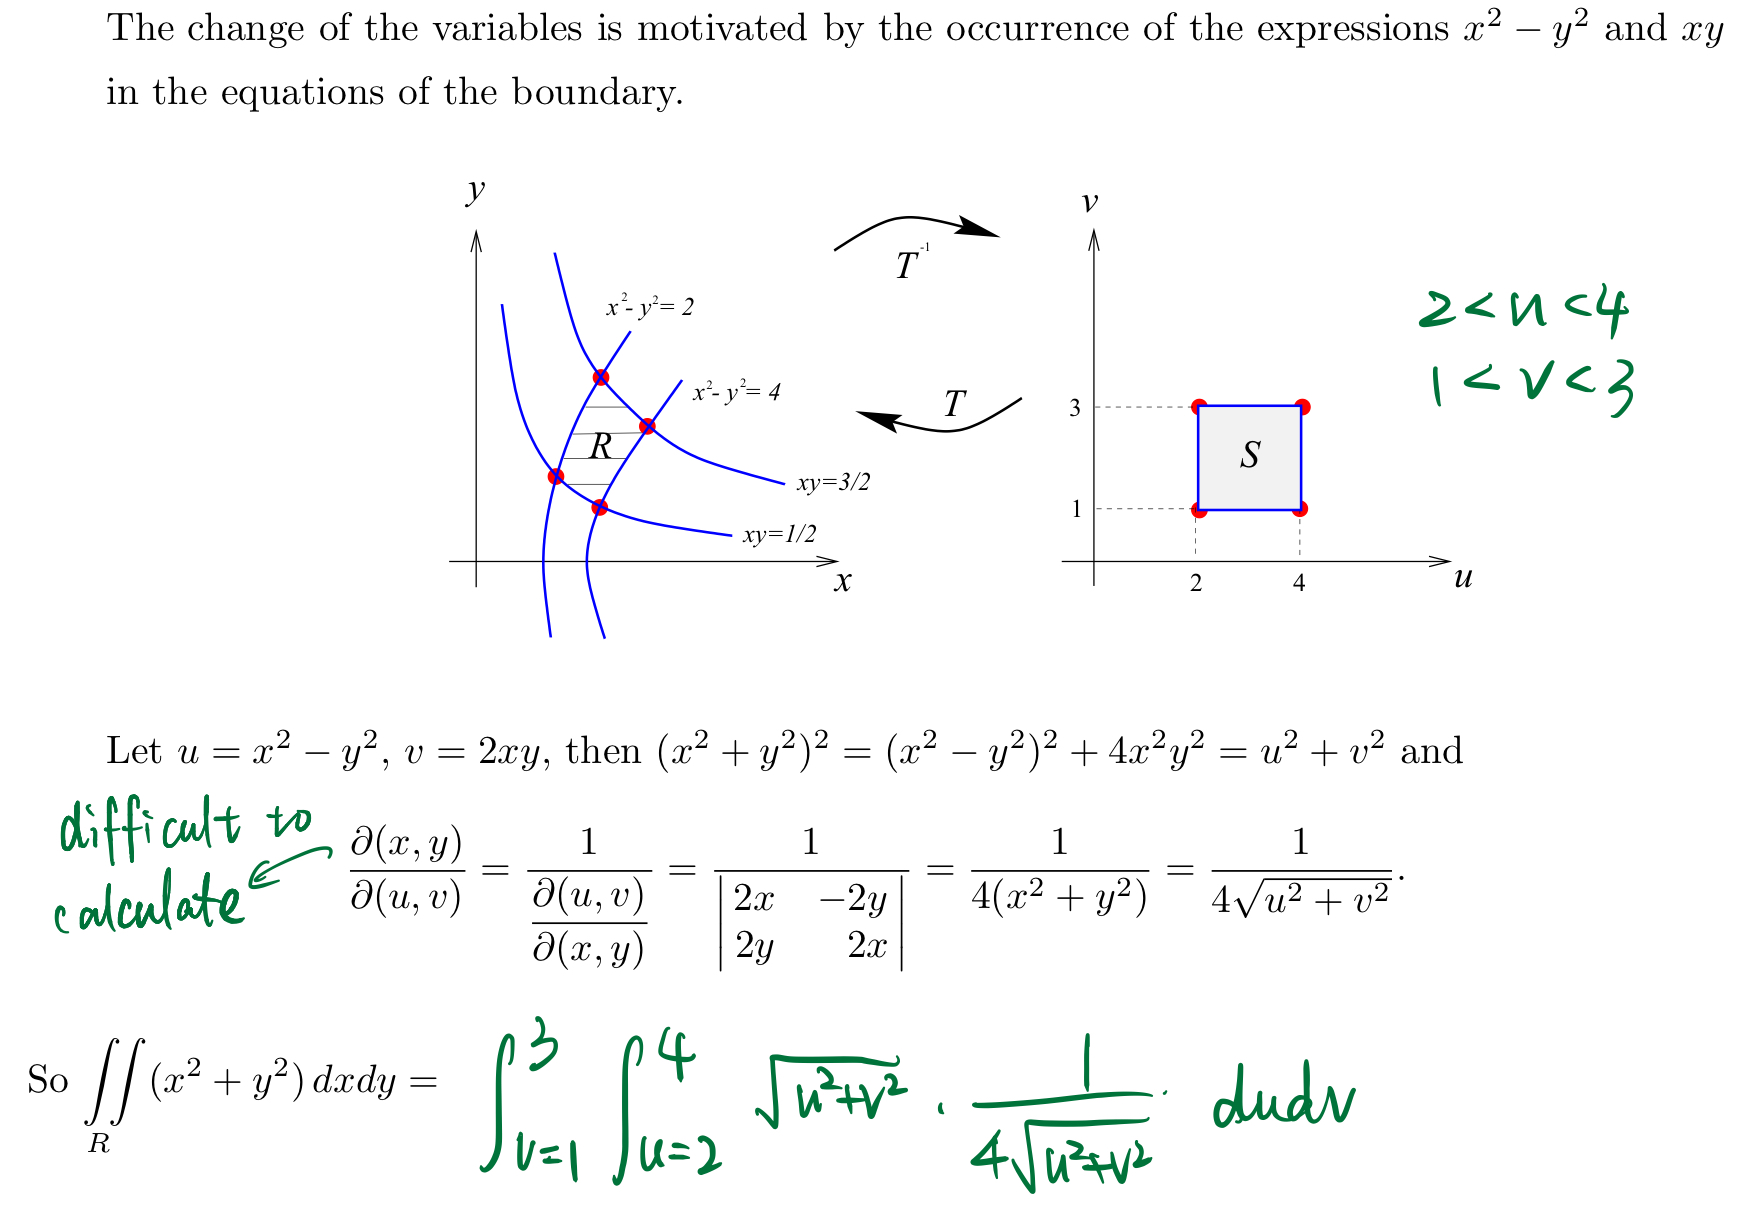
\includegraphics[scale=0.25]{images/Ch14-jacobian-eg3.jpeg}


    \newpage
    Sometimes, though the given region is a relatively good one, but it's still difficult to directly
    integrate, maybe because the integrand is too complicated. See the below example:

    \eg 
    
    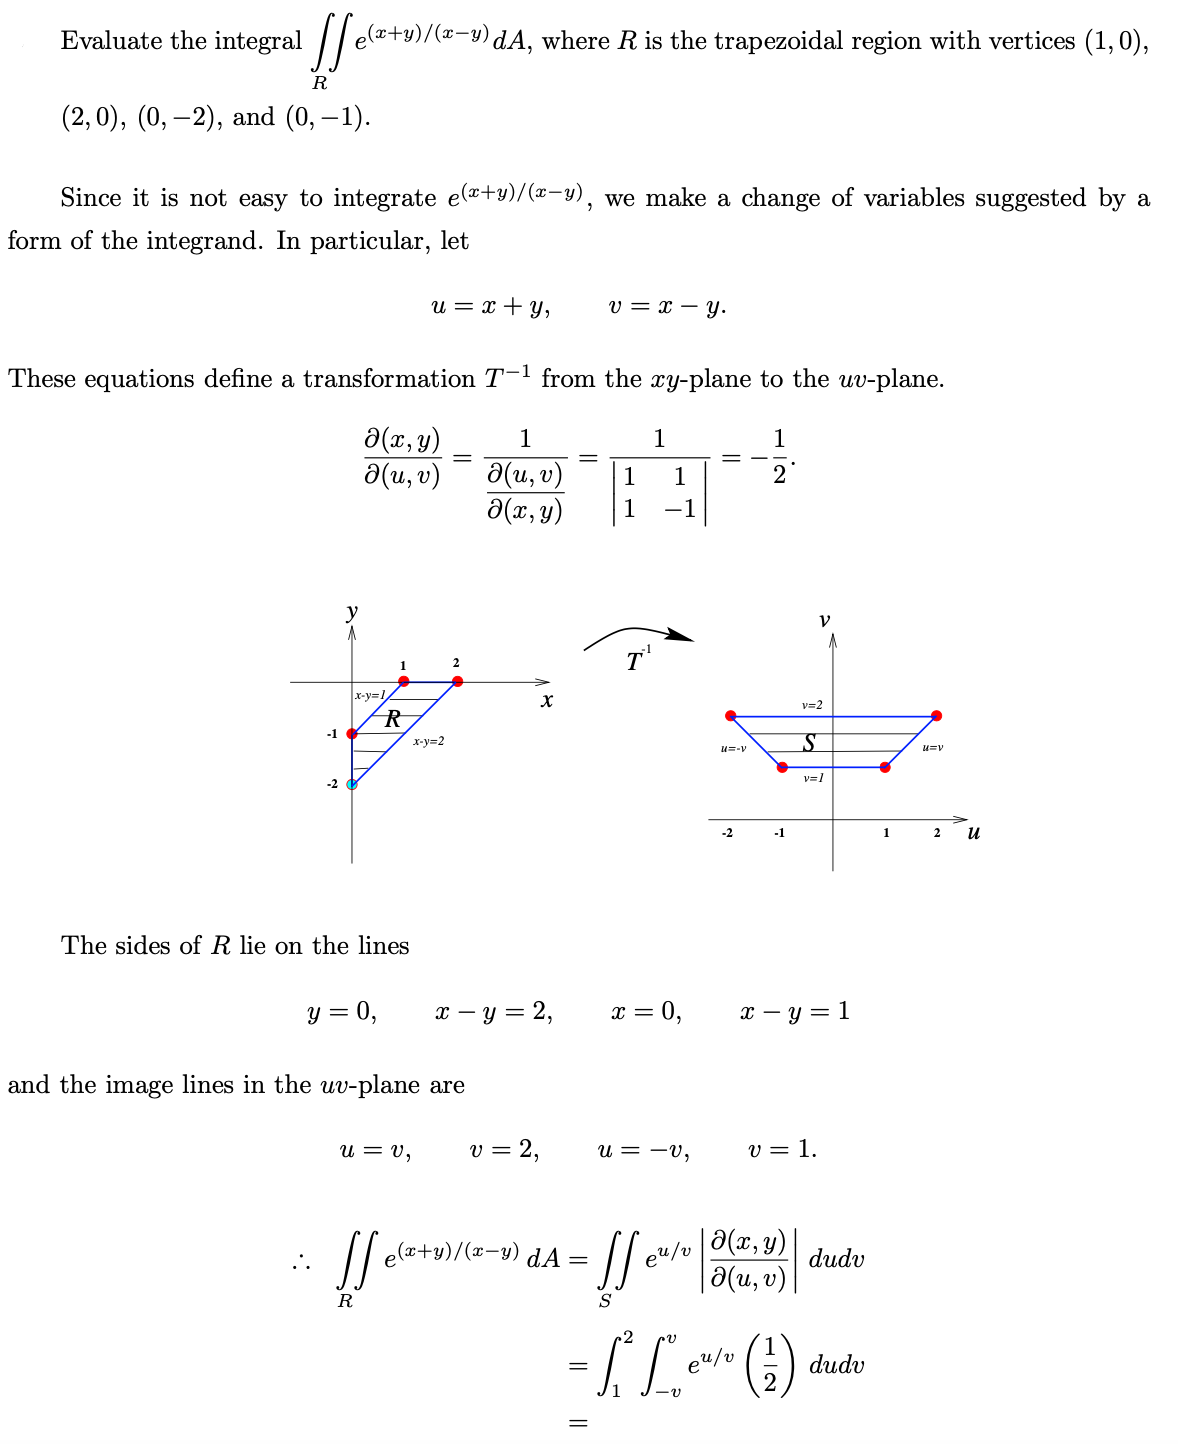
\includegraphics[scale=0.77]{images/Ch14-jacobian-eg4.png}
    


    \newpage
    \section{Surface Area}
    
    We now want to find the area of a surface. Finding an area on $xy$-plane is relatively easy, as we 
    have discussed early this chapter, but things become much more complicated when we are focusing
    on an arbitrary surface. So, we think about {\it projecting the area onto xy-plane}.

    \begin{center}
        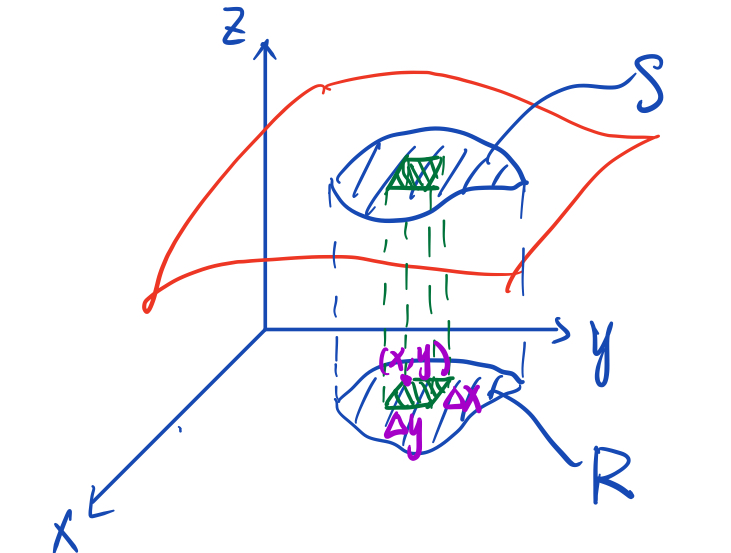
\includegraphics[scale=0.24]{images/Ch14-surface-area.jpeg}
    \end{center}

    As shown above, we want to find the area of region $S$ in a surface. The first thing to do 
    is to project it onto $xy$-plane, resulting in a region $R$.

    As usual, we use small rectangles to cover region $R$, as the green rectangle shown above,
    assume two sides are $\Delta x$ and $\Delta y$, so the area of green rectangle is $\Delta A
    =\Delta x\Delta y$.

    Then we project the rectangle up to the surface $S$, resulting in a ``curved-parallelogram''
    surface, shown as red area in left-below image. To find this area, we know as long as 
    $\Delta x$ and $\Delta y$ are small enough, the black parallelogram formed by $\Delta x$ and $\Delta y$
    is a good approximation for that area. By the way, the area of parallelogram is ${\bf u}\times {\bf v}$.

    How to represent ${\bf u}$ and ${\bf v}$? See the right-below image, the slope of vector ${\bf u}$
    is $\disp f_x=\dfrac{\Delta z}{\Delta x}$, so the width of ${\bf u}$ is $\Delta x$ and the height 
    of ${\bf u}$ is $\Delta z = \Delta x\cdot f_x$.(Notice this image is graphed vertically, i.e., 
    in $xz$-plane)


    \begin{center}
        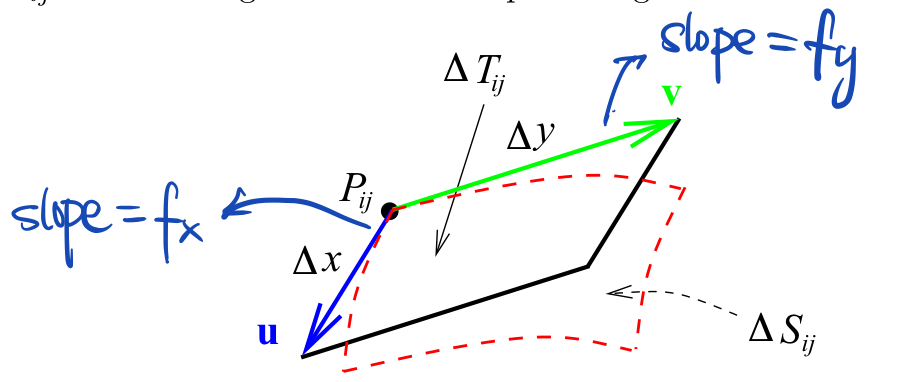
\includegraphics[scale=0.27]{images/Ch14-surface-area-vector.jpeg}
        \hspace{0.5in}
        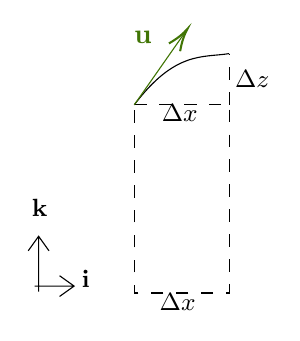
\begin{tikzpicture}[x=0.75pt,y=0.75pt,yscale=-1,xscale=1]
        %uncomment if require: \path (0,300); %set diagram left start at 0, and has height of 300

        %Shape: Rectangle [id:dp4999523728151394] 
        \draw  [dash pattern={on 4.5pt off 4.5pt}] (198,115.33) -- (243.67,115.33) -- (243.67,206.01) -- (198,206.01) -- cycle ;
        %Straight Lines [id:da4188949615125863] 
        \draw  [dash pattern={on 4.5pt off 4.5pt}]  (243.67,115.33) -- (243.67,90.67) ;
        %Curve Lines [id:da0065392042697955954] 
        \draw    (198,115.33) .. controls (217.67,89.34) and (231,92.67) .. (243.67,90.67) ;
        %Straight Lines [id:da5679442967275912] 
        \draw [color={rgb, 255:red, 65; green, 117; blue, 5 }  ,draw opacity=1 ]   (198,115.33) -- (222.52,80.31) ;
        \draw [shift={(223.67,78.67)}, rotate = 485] [color={rgb, 255:red, 65; green, 117; blue, 5 }  ,draw opacity=1 ][line width=0.75]    (10.93,-3.29) .. controls (6.95,-1.4) and (3.31,-0.3) .. (0,0) .. controls (3.31,0.3) and (6.95,1.4) .. (10.93,3.29)   ;
        %Shape: Axis 2D [id:dp1593594891661796] 
        \draw  (150,202.67) -- (169,202.67)(151.9,178.67) -- (151.9,205.33) (162,197.67) -- (169,202.67) -- (162,207.67) (146.9,185.67) -- (151.9,178.67) -- (156.9,185.67)  ;

        % Text Node
        \draw (209,205.07) node [anchor=north west][inner sep=0.75pt]  [font=\small]  {$\Delta x$};
        % Text Node
        \draw (245.33,97.4) node [anchor=north west][inner sep=0.75pt]  [font=\small]  {$\Delta z$};
        % Text Node
        \draw (210,114.07) node [anchor=north west][inner sep=0.75pt]  [font=\small]  {$\Delta x$};
        % Text Node
        \draw (196.67,78.73) node [anchor=north west][inner sep=0.75pt]  [color={rgb, 255:red, 65; green, 117; blue, 5 }  ,opacity=1 ]  {$\mathbf{u}$};
        % Text Node
        \draw (171.33,193.73) node [anchor=north west][inner sep=0.75pt]  [font=\small]  {$\mathbf{i}$};
        % Text Node
        \draw (147.33,159.73) node [anchor=north west][inner sep=0.75pt]  [font=\small]  {$\mathbf{k}$};
        \end{tikzpicture}

    \end{center}

    Therefore, ${\bf u}=\Delta x {\bf i}+0{\bf j}+\Delta x\cdot f_x{\bf k}$, 
    similarly, ${\bf v}=0 {\bf i}+\Delta y {\bf j}+\Delta y\cdot f_y{\bf k}$.
    Then $$||{\bf u\times v}||=||-\Delta x\Delta yf_x {\bf i}-\Delta x\Delta yf_y {\bf j}
    +\Delta x\Delta y {\bf k}||=\sqrt{(f_x)^2+(f_y)^2+1} \cdot \Delta x\Delta y$$

    When $\Delta x, \Delta y \rightarrow 0$, the area of $S$ is given by: 
    \begin{center}
        \boxed{$$\disp A=\iint_R \sqrt{(f_x)^2+(f_y)^2+1}\ dA$$}
    \end{center}
    

    \eg Given a plane $ax+by+cz=d$, where $a,b,c,d>0$. Find the area of the triangle bounded 
    by the intersections of the plane and axes.(As the red shaded area shown)

    \begin{center}
        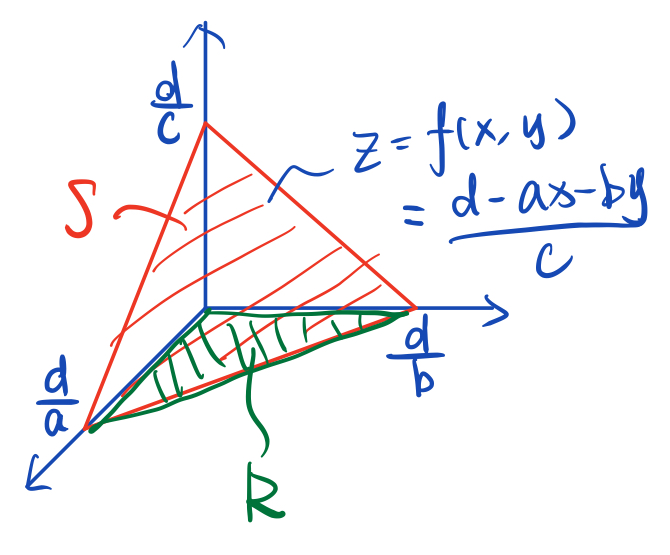
\includegraphics[scale=0.25]{images/Ch14-surface-area-eg1.jpeg}
    \end{center}

    \sol The equation of surface $z=f(x,y)$ is given by $z=\dfrac{d-ax-by}{c}$.

    To find the red area, we first {\it project it onto $xy$-plane}, resulting in green area $R$.

    Thus the red area $$S=\iint_R\sqrt{1+f_x^2+f_y^2}\ dA_{xy}$$

    We know that $f_x=-\dfrac{a}{c},\ f_y=-\dfrac{b}{c}$, so 
    $\sqrt{1+f_x^2+f_y^2}=\dfrac{\sqrt{a^2+b^2+c^2}}{c}$, then
    \begin{align*}
        S &= \iint_R{\blue \dfrac{\sqrt{a^2+b^2+c^2}}{c}}\ dA_{xy}\\
          &= \dfrac{\sqrt{a^2+b^2+c^2}}{c}\cdot {\rm (area\ of\ R)}\\
          &= \dfrac{\sqrt{a^2+b^2+c^2}}{c}\cdot \frac{1}{2}\cdot \frac{d}{a}\cdot \frac{d}{b}\\
          &= \frac{d^2\sqrt{a^2+b^2+c^2}}{2abc}
    \end{align*}
    Notice the blue part is a constant.

    \newpage
    \eg Find the surface area of the cone $z=\dfrac{h}{a}r$ (in cylindrical coordinate).
    \begin{center}
        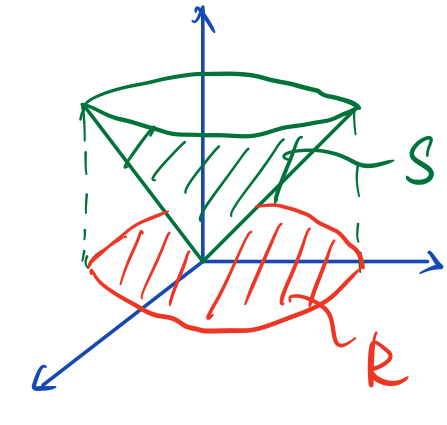
\includegraphics[scale=0.25]{images/Ch14-surface-area-eg2.jpeg}
    \end{center}

    \sol Project the cone onto $xy$-plane, resulting in red area $R$.

    The surface is given by $z=f(x,y)=\dfrac{h}{a}\sqrt{x^2+y^2}$

    Thus the green area $$S=\iint_R\sqrt{1+f_x^2+f_y^2}\ dA_{xy}$$

    We know that $f_x=\dfrac{h}{a}\cdot \dfrac{x}{\sqrt{x^2+y^2}},\ f_y=\dfrac{h}{a}\cdot \dfrac{y}{\sqrt{x^2+y^2}}$, so 
    $\sqrt{1+f_x^2+f_y^2}=1+\dfrac{h^2}{a^2}$, then

    \begin{align*}
        S &= \iint_R \sqrt{a+\frac{h^2}{a^2}}\ dA_{xy}\\ 
          &= \sqrt{a+\frac{h^2}{a^2}} \cdot {\rm (Area\ of\ circle\ with\ radius\ a)}\\
          &= \pi a\cdot \sqrt{a^2+h^2}
    \end{align*}

    \vspace{0.5in}
    \eg Find the area of the surface $z=x+y^2$ that lies above the triangle with vertices (0,0), (1,1)
    and (0,1).

    \sol 
    \begin{center}
        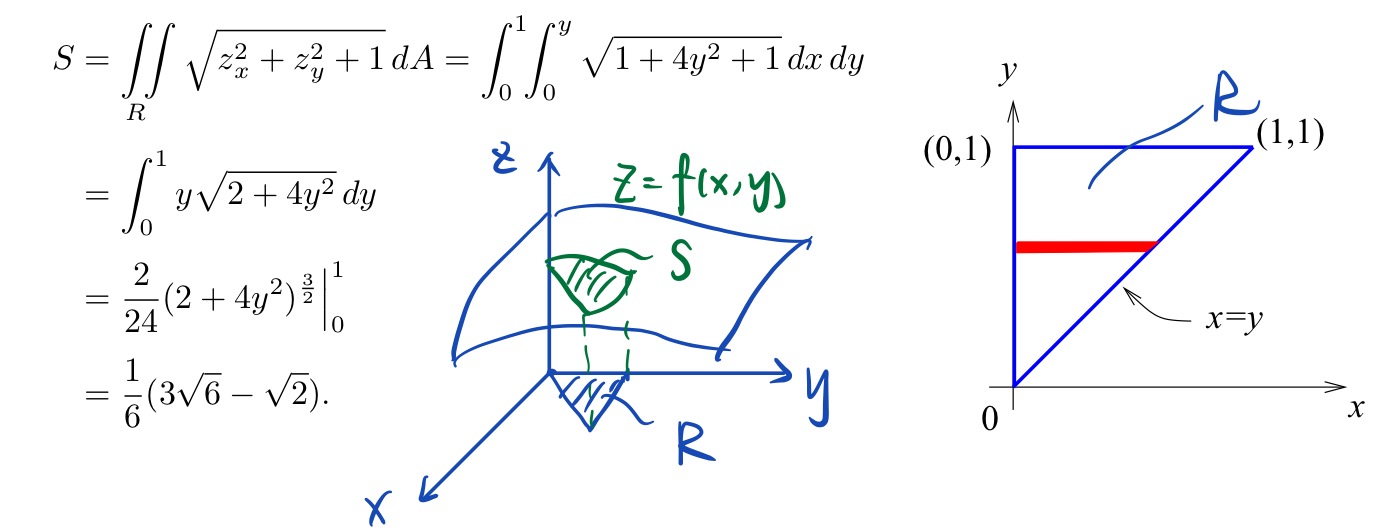
\includegraphics[scale=0.3]{images/Ch14-surface-area-eg3.jpeg}
    \end{center}


    \newpage
    \eg Find the surface of a sphere with radius $a$.
    \begin{center}
        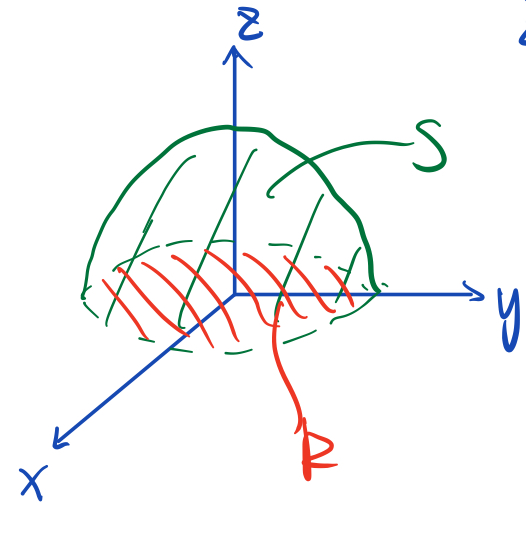
\includegraphics[scale=0.25]{images/Ch14-surface-area-eg4.jpeg}
    \end{center}

    \sol Again, project $S$ onto $xy$-plane to get region $R$.

    The equation of surface is given by $z=f(x,y)=\sqrt{a^2-x^2-y^2}$,
    
    The green area: $$S=\iint_R\sqrt{1+f_x^2+f_y^2}\ dA_{xy}$$

    We know that $f_x=\dfrac{-x}{\sqrt{a^2-x^2-y^2}},\ f_y=\dfrac{-y}{\sqrt{a^2-x^2-y^2}}$, so 
    $\sqrt{1+f_x^2+f_y^2}=1+\dfrac{x^2+y^2}{a^2-x^2-y^2}$, then
    $$S = \iint_R \sqrt{1+\dfrac{x^2+y^2}{a^2-x^2-y^2}}\ dA_{xy}$$
    Notice this integration is too difficult to calculate, so we consider using {\it polar coordinate}
    to substitute, let $r^2=x^2+y^2$, $dA=r\ drd\theta$, then 
    $$S = \iint_R \sqrt{1+\dfrac{r^2}{a^2-r^2}}\ r\ drd\theta=2\pi a^2$$

\end{spacing}
\end{document}
